\subsection{Cut-off and Saturation Regions:}

For the following experiment we assemble the circuit of Figure 3.3.0. The procedure consist in measure $V_{CE}$, $I_{B}$ and $I_{C}$ of {\bfseries\itshape 2N2222A} using three different resistors and different values for $V_{i}$. \hfill \break

{\bfseries\itshape\color{carmine}{Observation:}} {\itshape\color{carmine}{For each circuit we will explain which resistors and voltage were used.}} \hfill \break

\begin{multicols}{2}
\begin{figure}[H]
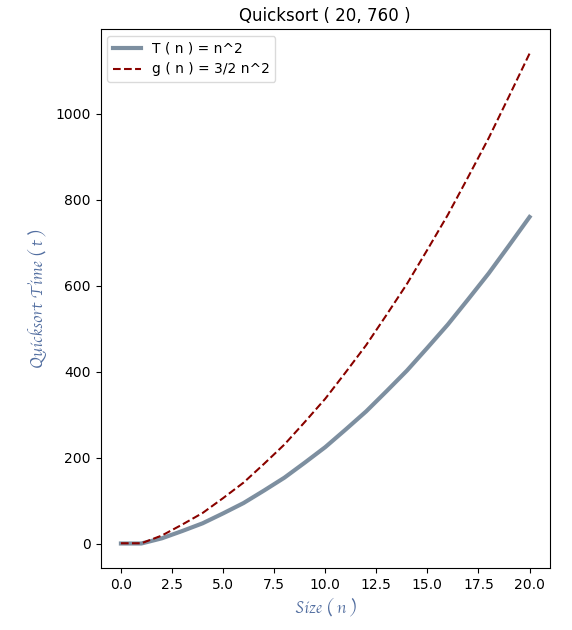
\includegraphics[scale=.8]{p2.png}
\centering \linebreak \linebreak Figure 3.3.0: Transistor in cutoff and saturation region.
\end{figure}

\begin{tasks}
\task For $V_{CE}$: The Collector-Emitter voltage can be measured by connecting the positive terminal of the voltmeter on the {\bfseries\itshape Collector} terminal, and the negative terminal of the voltmeter on the {\bfseries\itshape Emitter} terminal.
\task For $I_{B}$: The Base current can be measured by connecting the ammeter in series with {\bfseries\itshape $R_{B}$} and the {\bfseries\itshape Base} terminal of the transistor.
\task For $I_{C}$: The Collector current can be measured by connecting the ammeter in series with {\bfseries\itshape $R_{C}$} and the {\bfseries\itshape Collector} terminal of the transistor.
\end{tasks}
\end{multicols} \hfill \break

\begin{itemize}
\begin{multicols}{2}
\item For the first circuit we use $R_{C} = 100 \Omega$ and $R_{B} = 10K \Omega$, such that, we are going to prove it first with $V_{i} = 5 V$, once the values already mentioned were measured, we reduce $V_{i} $ to $0 V$ and we repeated the measures. The results were captured in the Table 3.

\begin{center}
\begin{tabular}[.5cm]{c c c}
\toprule
\toprule
\hspace{35pt} & \hspace{12pt} {\bfseries $V_{i}$ = 5 V} \hspace{12pt} & \hspace{12pt}  {\bfseries $V_{i}$ = 0 v} \hspace{12pt}  \\
\midrule
\midrule
$V_{CE}$ & 2.5 V & 12 V \\
\cmidrule{1-3}
$I_{B}$ & 0.420 mA & 0 A \\
\cmidrule{1-3}
$I_{C}$ & 89 mA & 0 V \\
\bottomrule
\linebreak
\end{tabular}
\linebreak Table 3: $R_{C} = 100 \Omega$ and $R_{B} = 10K \Omega$ resistor values circuit.
\end{center}
\end{multicols} \hfill \break

\begin{multicols}{2}
\item For the Second circuit we use $R_{C} = 100 \Omega$ and $R_{B} = 22K \Omega$, such that, we are going to prove it first with $V_{i} = 5 V$, once the values already mentioned were measured, we reduce $V_{i} $ to $0 V$ and we repeated the measures. The results were captured in Table 4.

\begin{center}
\begin{tabular}[1.5cm]{c c c}
\toprule
\toprule
\hspace{35pt} & \hspace{12pt} {\bfseries $V_{i}$ = 5 V} \hspace{12pt} & \hspace{12pt}  {\bfseries $V_{i}$ = 0 v} \hspace{12pt}  \\
\midrule
\midrule
$V_{CE}$ & 7.5 V & 12 V \\
\cmidrule{1-3}
$I_{B}$ & 0.204 mA & 0 A \\
\cmidrule{1-3}
$I_{C}$ & 45 mA & 0 V \\
\bottomrule
\linebreak
\end{tabular}
\linebreak Table 4: $R_{C} = 100 \Omega$ and $R_{B} = 22K \Omega$ resistor values circuit.
\end{center}
\end{multicols}
\end{itemize}

\pagebreak